%% pandoc template for the IEEE Transactions on Games version.
%% Class: IEEEtran.cls V1.8b (IEEE's LaTeX bundle IEEE-Transactions-LaTeX2e-templates-and-instructions.zip,
%% file IEEETransactions_LaTeX/IEEEtran/IEEEtran.cls), journal mode, after bare_jrnl.tex of that bundle.
%% Variables set by docs/manuscript_tog/tog.lua: abstract, indexterms; by the build command: classoption, runninghead.
\documentclass[journal]{IEEEtran}
\usepackage[T1]{fontenc}
\usepackage[utf8]{inputenc}
\usepackage{textcomp}
\usepackage{graphicx}
\usepackage{array}
\usepackage[hyphens]{url}
\usepackage[hidelinks,pdfusetitle]{hyperref}
\providecommand{\tightlist}{\setlength{\itemsep}{0pt}\setlength{\parskip}{0pt}}
\setcounter{secnumdepth}{2}
% let two-column figures and text share a page instead of leaving float-only pages half empty
\renewcommand{\dbltopfraction}{0.9}
\renewcommand{\topfraction}{0.9}
\renewcommand{\textfraction}{0.07}
\renewcommand{\dblfloatpagefraction}{0.85}
\renewcommand{\floatpagefraction}{0.85}
\setcounter{dbltopnumber}{3}
\hypersetup{pdfauthor={},pdftitle={A Frame-Only Census of Game Mechanics Built on ARC-AGI-3 Failed Preregistered Transfer Tests on MiniGrid/BabyAI and Procgen},pdfsubject={},pdfkeywords={},pdfcreator={},pdfproducer={}}
\begin{document}
\title{A Frame-Only Census of Game Mechanics Built on ARC-AGI-3 Failed
Preregistered Transfer Tests on MiniGrid/BabyAI and Procgen}
\author{Anonymous Author}
\markboth{Manuscript submitted to IEEE Transactions on Games}{Manuscript
submitted to IEEE Transactions on Games}
\maketitle
\begin{abstract}
I preregistered and tested the claim that a cheap description of game
mechanics, read from frames alone and frozen on eight games of
ARC-AGI-3, carries over to unseen games from two other benchmarks. It
did not. The description, an assumption census, reports for each game
whether five mechanical assumptions hold, such as one controlled object.
One registered test compared its verdicts with truth tables read from
each game's source code; a second asked whether its score predicts on
which games three frame-only agents complete the first level. The census
and the agents ran on 161 MiniGrid/BabyAI environments under two action
sets and on 14 Procgen games, 10,500 runs in all. By the registered
outcome table the result is a refutation, decided by the clause that the
validity test fails on any benchmark. The census failed that test for
three or four of the five assumptions on every tested benchmark and
condition, and no agent passed the prediction test. On all six primary
MiniGrid/BabyAI lines, a baseline fitted on grid area, action count and
color count ranked the games better than the census. An exploratory
reading suggests that the probes and the truth definitions were
different constructs.
\end{abstract}
\begin{IEEEkeywords}
Game-playing agents, general video game playing, benchmark mechanics,
preregistration, negative result.
\end{IEEEkeywords}
\section{Introduction}\label{introduction}

This paper reports a preregistered test and its negative answer. Before
any confirmatory run I registered the claim that a fixed, frame-only
description of a game's mechanics, built and frozen on one benchmark,
would describe games from two other benchmarks as their source code
does, and would predict, before any agent is run, on which of those
games agents that rely on the described mechanics finish the first
level. I tested both halves on MiniGrid/BabyAI and Procgen. By the
outcome table registered in advance, the claim is refuted: the
description failed the validity test on both benchmarks, and its score
passed the prediction test for no agent.

The question comes from agent evaluation on unseen games. A competition
that scores agents on games they were not built for {[}1{]} needs a
cheap way to say, before any agent is chosen, what the new games share
with the old ones. The agents studied here are frame-only: they see the
screen and are told when a level or the game ends, and receive no score,
no object list, no text and no game code. They carry built-in
assumptions about how games work, for example that one object on the
screen is the player and that the arrow keys move it one cell at a time.
Knowing which assumptions an unseen game satisfies would predict where
such agents finish the first level.

The assumption census was meant to supply that description. It is a
fixed set of probes that reads frames only and reports, for each game,
whether five mechanical assumptions hold. A1, input coupling, says that
the actions change the picture and that different actions change it
differently. A2, one controlled object, says that exactly one object on
the screen moves as a fixed function of the action. A3, lattice motion,
says that each movement action shifts that object by a constant step
whenever it is not blocked. A4, blocking by a fixed obstacle set, says
that whenever a move has no effect, a fixed set of obstacles explains
it, and that this set changes only through the agent's own actions. A5,
place goal, says that a level ends when the controlled object enters a
particular place, with no other condition at that moment. Each
assumption is a property of the game that can be read off its source
code. The census tries to infer them from play.

I set the census's parameters while developing a planner on eight of the
25 public games of ARC-AGI-3 {[}2{]}, and then froze them. The
registered protocol states that ARC-AGI-3 ``is the development instance
and does not count toward generality''. Transfer was to be shown on two
benchmarks the census had never been tuned on: MiniGrid/BabyAI, which
joins MiniGrid {[}3{]} and BabyAI {[}4{]}, and Procgen {[}5{]}. I
preregistered the claim because almost any reading of such an
instrument's output on new games can be made to look sensible after the
fact.

\section{Background and Related Work}\label{background-and-related-work}

\subsection{General Video Game
Playing}\label{general-video-game-playing}

Genesereth et al.~{[}6{]} define a general game playing system as one
that can accept a formal description of a game and play it effectively
without human intervention; their agents receive the rules. The General
Video Game AI (GVGAI) framework moved the problem toward games whose
rules the agent is not shown. The first General Video Game Playing
Competition asked for a single agent that can play many different games,
some of them unknown to the entrants when they submitted, and left it to
the agents to discover the mechanics of each game {[}1{]}. Perez-Liebana
et al.~{[}7{]} describe the framework as games written in the Video Game
Description Language and tracks in which agents play unknown games with
or without access to a simulation of the game. The agents studied here
sit at the end of that range with the least information: no rules, no
simulation and no score, only frames and the signal that a level has
ended.

\subsection{Evaluating Agents on Unseen
Games}\label{evaluating-agents-on-unseen-games}

An evaluation on unseen games is only as informative as what is known
about how those games differ from the ones an agent was built on. Legg
and Hutter {[}8{]} take intelligence to measure an agent's ability to
achieve goals in a wide range of environments, which makes the range
part of what a score means. Chollet {[}9{]} argues that skill at a given
task falls short of measuring intelligence, because unlimited priors or
training data can buy arbitrary levels of skill, and presents the
Abstraction and Reasoning Corpus (ARC). Game benchmarks answer the same
concern with held-out content: Procgen generates levels procedurally so
that agents can be trained and tested on different levels {[}5{]}, and
BabyAI and MiniGrid offer families of grid tasks {[}4{]}, {[}3{]}. None
of them describes, game by game, which mechanical assumptions hold; the
census was an attempt to do so from frames.

\subsection{Predicting Agent Success From Game
Properties}\label{predicting-agent-success-from-game-properties}

The closest earlier attempt, Bontrager et al.~{[}10{]}, reported a
mainly negative result. They read mechanics features from the rule files
of general video game playing games. A clustering of the games by those
features agreed poorly with a clustering by controller performance, and
the authors concluded that the features were not good indicators of
performance. A selection agent built on two of the features did beat
each of its constituent controllers on the same games. One possible
objection to that design is that features read from rules say nothing
about whether an agent could perceive them. Another is that the target,
the best controller from a portfolio, was not tied to any assumption the
features express. This study was designed to meet both objections. The
census measures its features from frames, as an agent would; its
accuracy against source-derived truth is tested separately, as test V1;
and its prediction target, first-level completion by a stated class of
agents that rely on the assumptions, is tested as V2, registered before
any run. Two other lines of work predict success from different
information. Gaina et al.~{[}11{]} predict wins on held-out games from
an agent's own experience during play, not before it. Laidlaw et
al.~{[}12{]} predict the sample complexity of deep reinforcement
learning from a property of the full tabular decision process with its
reward, which a frame-only agent does not have.

\subsection{ARC-AGI-3 and Frame-Only
Agents}\label{arc-agi-3-and-frame-only-agents}

ARC-AGI-3 is an interactive benchmark of turn-based environments that
come without explicit instructions; each environment is a series of
levels, and at each turn the agent sees a frame, a grid of 64 by 64
cells in 16 possible colors, and takes one action {[}2{]}. Its public
demonstration set has 25 environments, and the report states that this
set does not cover all the mechanics found in the private set. Rudakov
et al.~{[}13{]} published a graph-based explorer for these games, which
is one of the agents used here. Liew {[}14{]} classifies the public
games by the simplest strategy without reasoning that reaches a level, a
classification that concerns reachability rather than mechanics and
makes no registered prediction. Skoutnev et al.~{[}15{]} identify goals
with a coding agent built on a large pretrained model, which writes an
executable world model of each game and so brings a learned prior; that
places it outside the prior-free class studied here.

\subsection{Finding the Controlled
Object}\label{finding-the-controlled-object}

Bellemare et al.~{[}16{]} brought contingency awareness into
reinforcement learning, defining contingent regions as the parts of an
observation whose next value depends on the agent's action, and Choi et
al.~{[}17{]} learned controllable regions with a neural network. A1 and
A2 take that idea and replace the learned components with fixed counting
rules.

\subsection{Holdout Reuse and
Preregistration}\label{holdout-reuse-and-preregistration}

When the same held-out set is consulted again and again while choices
are made, choices can come to fit it {[}18{]}; Roelofs et al.~{[}19{]}
measured this effect across many machine learning competitions and found
little of it. The study kept a fixed split of the ARC-AGI-3 games, and
kept the two confirmatory benchmarks out of development altogether.
Bertinetto et al.~{[}20{]} describe a model of preregistration for
machine learning research, in which the experimental protocol is fixed
and reviewed before the experiments are run. This protocol follows that
model without the review: it was fixed, tagged in the repository and
registered on the Open Science Framework before any confirmatory game
was played.

\section{Method}\label{method}

The file and line of each registered constant, the full amendment trail,
the exclusion lists and the hashes of the frozen files are in the
supplement. Repository addresses, commit hashes, registration addresses
and preprint identifiers are withheld in this version for
double-anonymous review.

\subsection{The Instrument}\label{the-instrument}

The census reads the run of the planner N (Section III-D) on a game for
20,000 actions per seed: the frames and the signals that a level or the
game has ended, and nothing else. From the planner's report at the end
of the run it makes five decisions per seed, with rules written into the
registered protocol and implemented in the frozen analysis code. A1
holds when some key has a learned shift and the tried keys' shifts are
not all equal. A2 holds when some key was accepted as moving one object
and the planner located that object. Acceptance needs three agreeing
presses with a margin of 2:1 over the next most frequent displacement.
A3 holds when A2 holds and the planner's model of the first level did
not end in a failure of prediction or localization. A4 holds when A3
holds and the planner never walked through a color it had classified as
a wall. A5 holds when a place recorded at a level end later ended a
level again. It fails when such a place was reached without a level end
and never confirmed, and it is undetermined otherwise. The verdict for a
game is the majority over its 10 seeds: it holds if at least half of the
seeds say so, else it fails if at least half say so, else it is
undetermined.

I froze every parameter of the census before registration and copied
each into the protocol from its source file. They include three agreeing
presses to accept a key, the 2:1 margin, at most eight presses per key
while learning, a planner search limit of 40000 nodes, and a motion
detector that needs at least 2 changed cells. Six files hold the census
and its two agents. Their git blob hashes are registered (Supplement,
Section S.6), and the runner refused to start if any of them differed.

I set these parameters while developing the planner on eight ARC-AGI-3
training games, and kept the other 17 public games as a held-out set
whose source code I never opened. The split file held 18 games in the
held-out set until 21 September 2026, when I moved one of them, dc22, to
the development set to debug the agent's wall learning on it. The
protocol provided for a truth table derived from source for the eight
development games, and for V1 on them, labeled development, once that
table existed. I never wrote the table, so the census was never scored
against source-derived truth on its development instance. The registered
ARC-AGI-3 baseline ran my agents R and N on all 25 public games with 10
seeds and 20,000 actions under the registered code, 500 runs in all.

\subsection{The Benchmarks and How Each Is
Presented}\label{the-benchmarks-and-how-each-is-presented}

The frozen code presses six key identifiers only, so every benchmark is
presented through a fixed key map of at most six actions. On
MiniGrid/BabyAI (minigrid 3.1.0, gymnasium 1.3.0, Python 3.11.9) there
are two conditions. Under primitive actions the keys are turn left, turn
right, forward, pickup, drop and toggle. Under absolute moves they are
north, south, west and east, each a turn to face that direction followed
by a step forward, plus pickup and toggle. The action ``done'' is
offered in neither condition. The grid is rendered with 8 × 8 pixel
tiles, each distinct tile pattern receives an integer index, the four
orientations of the agent's triangle are merged into one index, and the
grid is placed at the top left of a 64 × 64 canvas, one row down,
because the frozen code reads rows 1 to 62 only.

On Procgen (procgen 0.10.7, Python 3.10, easy mode, sequential levels)
the keys are up, down, left, right and two special actions. Frames are
64 × 64 color images, mapped to integer indices by exact color. The
frozen code does not see the top and bottom pixel rows, which was
recorded and not corrected. The primary condition draws the whole level
into the frame (center\_agent off), where the agent can be very small,
and the census detects motion only when at least 2 cells change. The
protocol therefore registered an operating range before any run, the
games whose agent spans at least 2 pixels: nine of the 14 confirmatory
games, and Procgen results are reported over all 14 and over these nine.
The secondary condition, a view centered on the agent, is identical to
the primary one on the ten Procgen games that set the camera option
themselves at every level start, nine of them confirmatory and exactly
the nine in the operating range; a camera check found 401 of 401 frames
identical there. The secondary condition is therefore distinct on five
confirmatory games only, and it is reported there and never tested.

\subsection{Truth From Source}\label{truth-from-source}

Each benchmark has a truth table, committed before the protocol was
registered, with one line per environment, read by hand from the
installed minigrid 3.1.0 source (per environment class, its step
function or instruction verifier) and from the Procgen C++ source at tag
0.10.7. Each entry names the file and line that justify it, and the
definitions of A1 to A5 used by the truth tables are written out in the
protocol. Under primitive actions A3 fails on every MiniGrid/BabyAI
environment, because the displacement of forward depends on which way
the agent faces. On the 161 confirmatory MiniGrid/BabyAI environments,
A1, A2 and A3 under absolute moves hold everywhere, A4 fails on 5 and A5
holds on 36. On the 14 confirmatory Procgen games, A2 holds on 6, A3 on
2, A4 on 13 and A5 on 6. The truth tables are the registered answer key
of test V1; the census is the instrument under test.

\subsection{Agents}\label{agents}

Three agents ran on every game, seed and condition. R, my explorer,
tries actions and records the frames it has seen; it is evidence for V2.
N, my planner, learns a step vector for each key, locates the controlled
object, plans toward unexplored places and tests goal hypotheses; it
uses the five assumptions by construction, so its V2 lines are an
instrument check only, and its runs supply the census. I1 is the
graph-based explorer of Rudakov et al.~{[}13{]}, run unchanged behind a
boundary adapter, and it is evidence for V2. I1's own code maps five
actions, so it has no toggle on MiniGrid/BabyAI and no second special
action on Procgen.

\subsection{Registration and Amendment
Trail}\label{registration-and-amendment-trail}

I registered version v1 of the protocol on 27 September 2026 as git tag
prereg-v1 in the study's repository, and on the same day on the Open
Science Framework (OSF) as an open-ended registration. It fixed the
claim, the agents, the census rules and constants, the truth tables, the
benchmarks and their splits between pilot and confirmatory games, the
seeds and budget, the tests and thresholds, the analysis code and the
outcome table. The registered claim, in the OSF text, reads:

\begin{quote}
A fixed, cheap, frame-only probe battery (the assumption census: A1
input coupling, A2 one controlled object, A3 lattice motion, A4 blocking
by a fixed obstacle set, A5 place goal), with every parameter frozen on
eight ARC-AGI-3 training games, (i) reports the ground-truth mechanics
of unseen games at a registered accuracy, and (ii) predicts, before any
agent is run, on which unseen games assumption-driven frame-only agents
complete the first level. Ground truth is derived from each game's
source code and committed before any run. A goal-identification cost G
is measured and reported alongside, not tested. ARC-AGI-3 is the
development instance and does not count toward generality.
\end{quote}

The git-tagged protocol words the claim differently: it names G as part
of the battery and says ``in three suites''; the tests, thresholds and
outcome table are the same in both texts. G counted level ends until one
goal hypothesis was left. Its elimination over places is the
singletons-plus-empty example of Goldman and Kearns {[}21{]}, in
complement form, and its elimination over features is version-space
elimination in the sense of Mitchell {[}22{]}. Goal recognition design
{[}23{]}, {[}24{]} is related but concerns an outside observer of an
actor's goal, whereas G concerns a learner's own goal.

The pilot games, six MiniGrid/BabyAI environments and two Procgen games,
could be run before the confirmatory set and are excluded from every
confirmatory analysis; the pilot could change adapter code, logged in
the next version's dated diff, but never a census constant, threshold,
truth entry or frozen file. After the pilot I registered version v1.1 on
27 September 2026 as git tag prereg-v1.1, and on the same day on the
OSF. Both registrations have been public since 14 October 2026, when I
ended their embargoes. I wrote version v1.2 after the outcome and tagged
it prereg-v1.2 on 13 October 2026.

The amendment trail has 16 entries, D1 to D16, given in full in
Supplement, Section S.3. D1 to D15 form the v1.1 diff, written on 27
September 2026 after the pilot and before any confirmatory game was
played; they fix how each benchmark is presented through the six-key
limit, the time caps, the runner, the boundary of I1, the checks, the
exclusions from V2, the analysis code, the Procgen camera identity and a
replay planned for G. D16, the only entry of v1.2, written after the
outcome, withdraws G without measuring it. No threshold, parameter,
exclusion list, truth entry or analysis script changed after the
prereg-v1.1 tag.

\subsection{Tests and Thresholds}\label{tests-and-thresholds}

Test V1, instrument validity, compares the census's game verdict with
the truth table, per benchmark, condition and assumption, over the
confirmatory games. It passes when the share of agreeing games is at
least 0.90 and Cohen's kappa is at least 0.70. It fails when agreement
is below 0.75, and anything between is ``neither''. Kappa is computed
only where both truth values have at least 3 games; elsewhere agreement
decides alone. An undetermined census verdict never counts as agreement,
and for kappa it is mapped to the value opposite the truth. That
treatment of ``undetermined'' is in the registered text, which reads
``An `undetermined' census never agrees. For {[}kappa{]} it is mapped to
the value opposite the truth.'' (The registered text has the Greek
letter where the brackets stand.) The frozen analysis code at the tag
implements the same rule.

Test V2, predictive validity, works per benchmark, condition and agent.
Each game has a census score, the number of the five assumptions whose
verdict holds (undetermined does not hold). It also has a conjunctive
prediction, that A2, A3, A4 and A5 all hold, and an outcome: the agent
completed the first level in at least half of its 10 seeds. The score is
judged by the area under the receiver operating characteristic curve
(AUROC) for the outcome. V2 passes when four conditions all hold. The
AUROC is at least 0.80. The lower end of its 95\% bootstrap interval,
from 2,000 resamples of games with seed 20260927, is above 0.60. The
balanced accuracy of the conjunctive prediction is at least 0.80. The
AUROC exceeds that of a nuisance baseline by at least 0.10. V2 fails
when the AUROC is at most 0.65, and the test is void when the share of
games completed lies outside {[}0.10, 0.90{]}. The nuisance baseline, a
logistic regression of the outcome on grid area, number of actions and
number of palette colors fitted in-sample, asks whether the census adds
anything to the size and variety of a game. Evidence comes from R and
I1, and a benchmark fails V2 when every non-void evidence agent fails.
On MiniGrid/BabyAI the registered text tests V2 under absolute moves and
reports it under primitive actions. On ARC-AGI-3, V2 on the 17 held-out
games is reported and not tested.

Test V3, parameter transfer, requires every census constant and frozen
file to be identical on every benchmark, registered as a check of the
adapter and code fields of every row. The analysis code does not compute
it (Section III-J); what the record shows is that the runner compared
the six frozen files with their registered hashes before each
confirmatory block, refused to start on any difference, and logged all
six matching for both blocks.

The protocol fixed three outcomes and the venue that each would allow,
before any confirmatory run. Support needed V1 to pass on both
benchmarks and V2 to pass for R and I1. Partial needed V1 to pass
everywhere with a weaker V2. Refute follows when V1 fails on any suite,
or V2 fails on MiniGrid/BabyAI under absolute moves, or V2 is void on
every suite. Its registered venue is ``repository record only, at most
an arXiv note''. The table is reproduced in Section IV (Table III).

\subsection{Exclusions From V2}\label{exclusions-from-v2}

The registered rule (D9) excludes an environment from an agent's primary
V2 line when, on every seed, success cannot be reached without an action
missing from that agent's map. The action may trigger success, or it may
be a precondition of every successful episode. One environment has no
success at all and is excluded for every agent. For R and N the rule
excludes 6 environments under primitive actions and 49 under absolute
moves, leaving 155 and 112. In the pilot, I1, which has no toggle,
completed no level on a locked-door environment in any of its 20 runs.
D9b therefore applied the same rule to I1's own key map, adding the 57
environments where success needs toggle on every seed. I1's primary
lines exclude 63 and 78 environments, leaving 98 and 83. Procgen has no
exclusion. Lines with the excluded environments included are reported
and not tested. The lists, with identifiers, are in Supplement, Section
S.4.

\subsection{Seeds, Budget and Caps}\label{seeds-budget-and-caps}

Every agent ran with seeds 1000 to 1009 and a budget of 20,000 actions
per game, seed and condition. The wall-clock cap per run was three times
the longest pilot run: 3300 s on MiniGrid/BabyAI, where the longest
pilot run took 1081.6 s, and 7500 s on Procgen, where it took 2481.5 s.
The cap for the ARC-AGI-3 baseline was 3600 s. There were 9,660
confirmatory runs on MiniGrid/BabyAI (161 environments, 2 conditions, 3
agents, 10 seeds) and 840 on Procgen (14 games, 2 conditions, 3 agents,
10 seeds), 10,500 in all. Every run reached its budget, with 0 errors
and 0 runs cut by the cap. The MiniGrid/BabyAI block ran on one CPU
machine; it started on 28 September 2026 and had finished by 13 October
2026.

\subsection{Checks Before and After the
Runs}\label{checks-before-and-after-the-runs}

Four infrastructure checks were registered, and none computes a census
or a test statistic. A fidelity check played 200 random actions twice
per game and condition and found identical frames in 334 of 334
comparisons on MiniGrid/BabyAI and 32 of 32 on Procgen. A pilot check
read the 480 pilot runs and found 0 errors and 0 runs short of the
budget, and 0 confirmatory configurations projected over their cap. The
camera check is described above. A determinism check compared, on the
nine Procgen games where the two camera conditions draw the same frames,
every secondary run with its primary run: all 270 of 270 pairs were
identical in every field except timing and the condition labels. The
analysis code and the determinism check passed 20 of 20 synthetic tests
at the tag before the analysis read any confirmatory row.

\subsection{Deviations From the Registered
Protocol}\label{deviations-from-the-registered-protocol}

Eight departures from the registered protocol, or from what it implies,
are recorded here. None changes a test, a threshold or the outcome. The
first is D16, written on 13 October 2026, after the outcome was known.
The registered claim says that the goal-identification cost G is
``measured and reported alongside, not tested'', and D16 withdrew G
without measuring it, because the instrument it accompanies had failed
V1.

The second concerns the venue. The registered consequence of a
refutation is ``repository record only, at most an arXiv note''. On 13
October 2026, with no arXiv endorsement available to me, I recorded that
the clause would be read as ``at most a preprint'' and that no journal
submission would follow. After the preprint drafts of 14 October 2026 I
reversed the second part and chose to seek peer review of the negative
result. An earlier version of this article is a preprint on Zenodo, and
this version is submitted to IEEE Transactions on Games. This changes no
analysis and no number.

The third is a defect in the frozen analysis code, found on 13 October
2026 and recorded, not corrected. The code computes the two ARC-AGI-3
lines of V2 over all 25 public games, the eight development games
included, instead of over the 17 held-out games. It also prints a
per-agent verdict on them that has no registered meaning. The fourth is
an omission rather than a departure. The pilot runs contained census
verdicts for eight games that have truth-table entries, and a V1
comparison on them before the v1.1 tag could have shown the failure
before the confirmatory runs. It was not registered and I did not make
it; I recorded it as a lesson on 13 October 2026. The fifth I found on
14 October 2026, while writing an earlier version of this article. The
registered text tests V2 on MiniGrid/BabyAI under absolute moves and
only reports it under primitive actions, but the frozen code prints
verdicts, and a suite line, for the primitive-action lines as well.
Those verdicts enter no outcome clause.

The last three I also found on 14 October 2026, while reviewing that
earlier version against the protocol. The sixth: v1 provided for a truth
table of the eight ARC-AGI-3 development games and for V1 on them,
labeled development, once the table existed. The record listed the table
as still outstanding at the v1.1 tag, and I never wrote it. The seventh:
v1 listed I1 among the agents to run on ARC-AGI-3, but the registered
ARC baseline ran R and N only. The eighth: V3 was registered as a check
of every row's adapter and code fields, and the analysis code never
computed it. The ARC-AGI-3 lines are reported and not tested, and V3
matters only for the outcome Support, so none of these three changes the
outcome.

\section{Results}\label{results}

The results are the registered tests exactly as the frozen analysis code
wrote them; where the code prints a verdict that the registered text
does not test, the text says so. Tables I and II give the verdict of
each line, and the full tables, with every statistic, are in Supplement,
Sections S.1 and S.2.

Fig. 1 and Table I give V1. On MiniGrid/BabyAI under absolute moves, A1
and A2 pass and A3, A4 and A5 fail. Under primitive actions only A1
passes; A2, A3, A4 and A5 fail. On Procgen with the whole-level view,
over all 14 games, A1 passes and the other four fail. On the nine
in-range games, A1 is ``neither'', with agreement 0.8889, and A2 to A5
fail. The camera-on condition is reported and not tested. Cohen's kappa
is negative for A5 under absolute moves (-0.4125), under primitive
actions (-0.3374) and on Procgen (-0.7843), and for A4 under absolute
moves (-0.0435).

\begin{figure*}[!t]
\centering
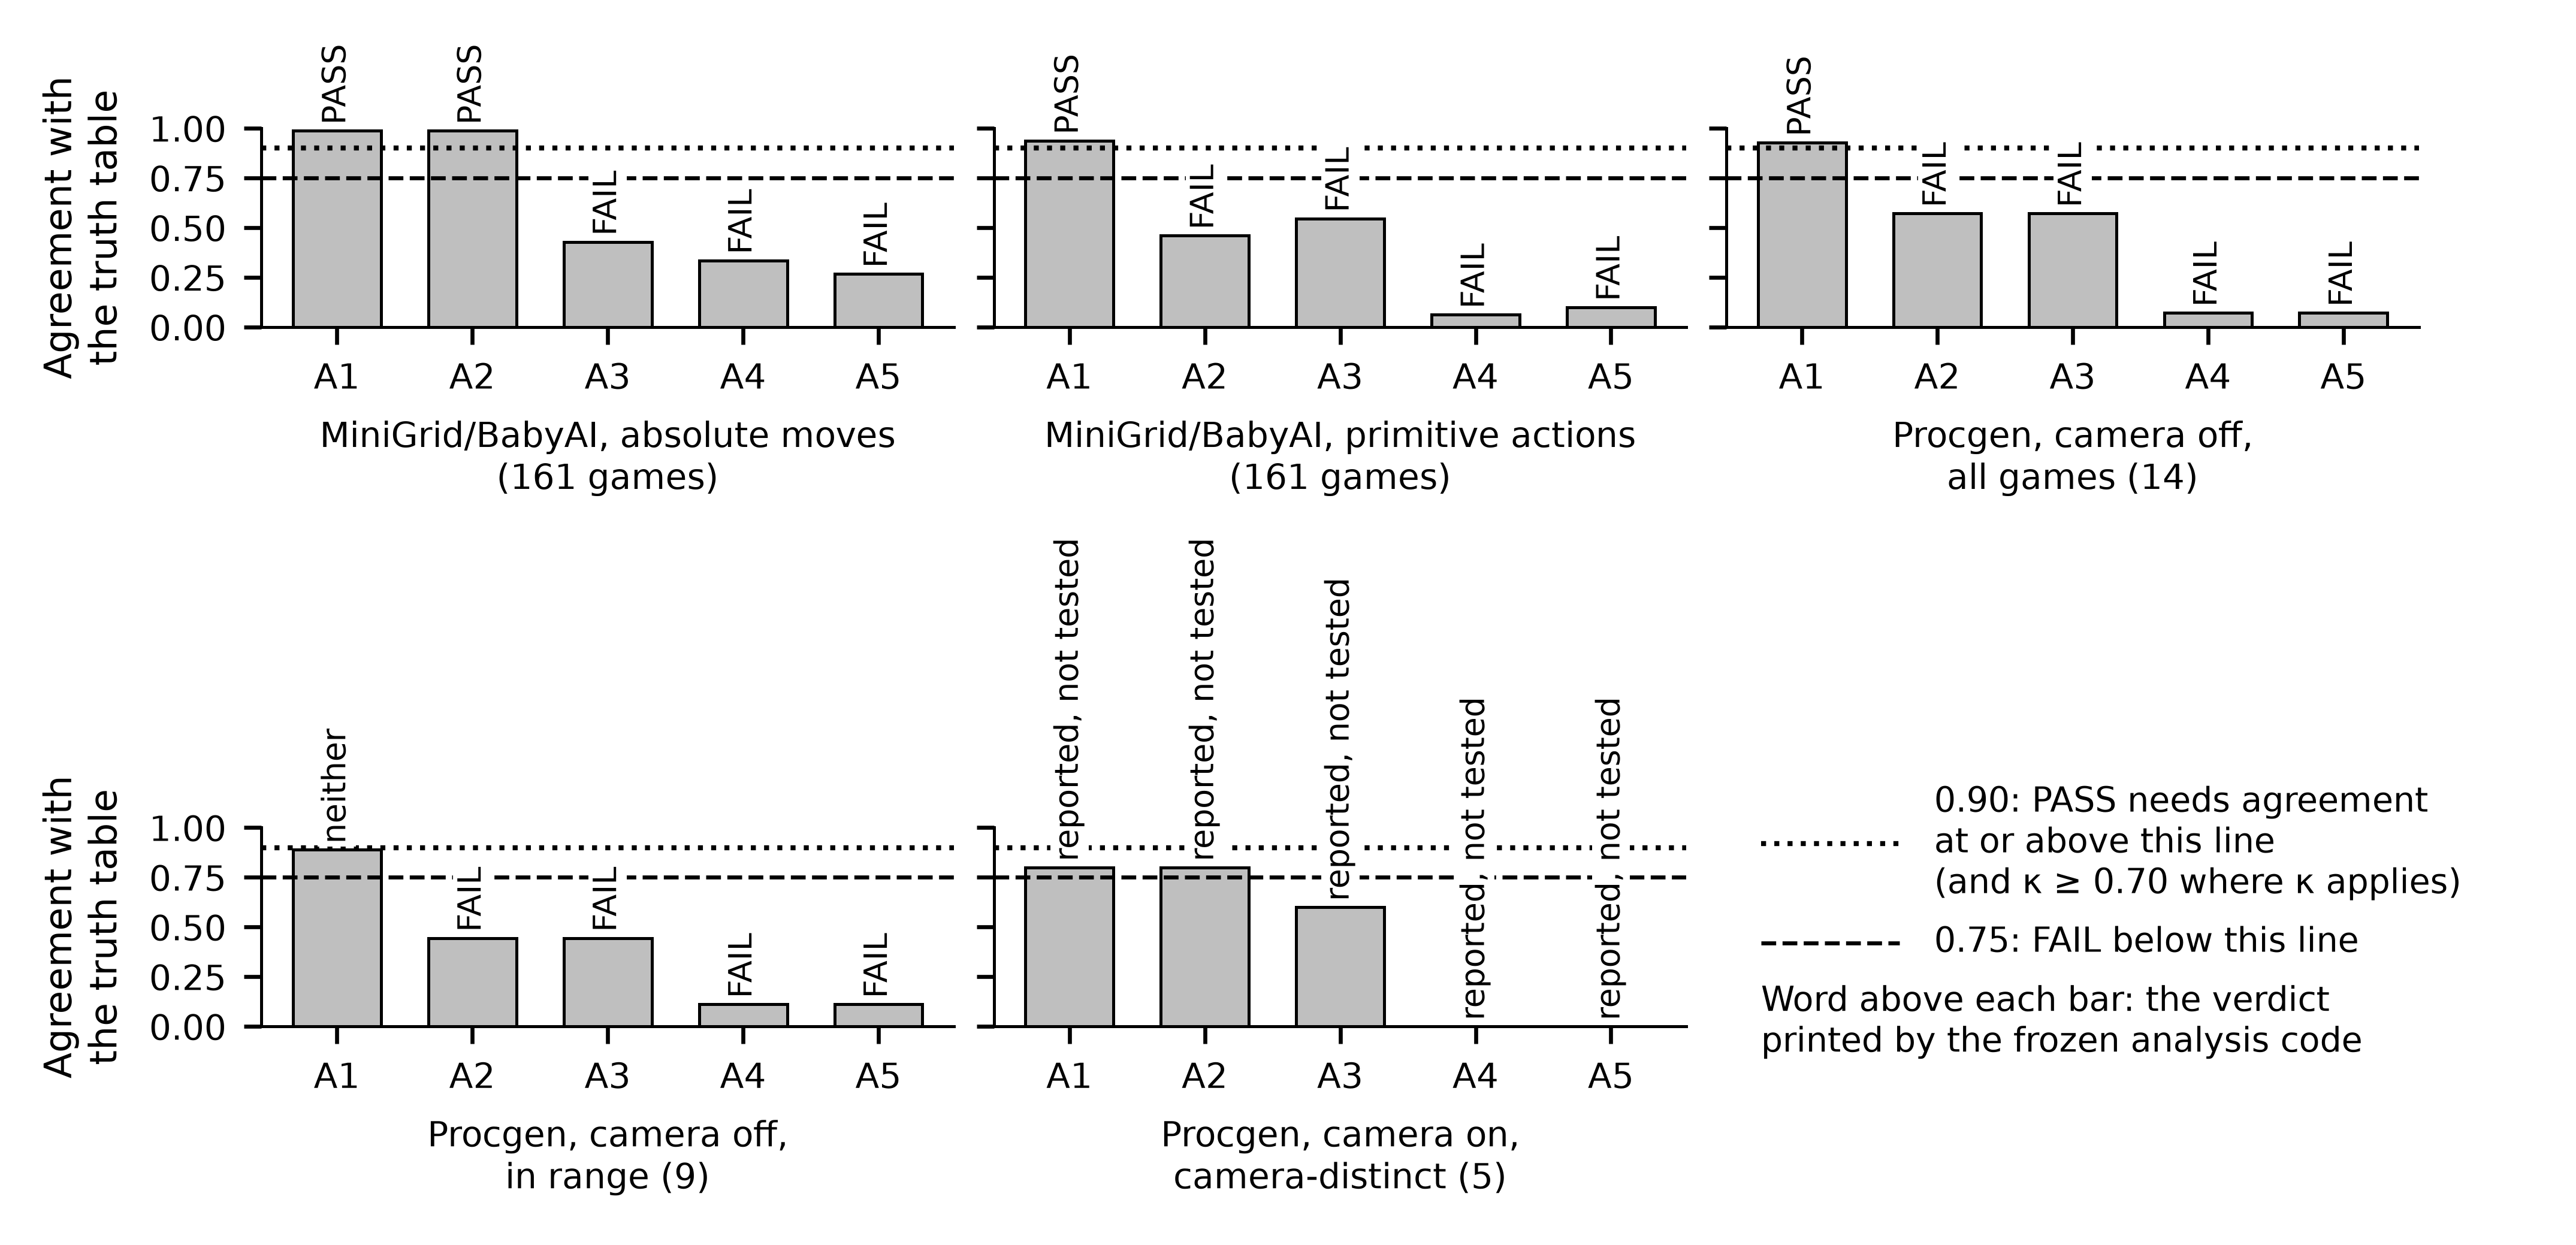
\includegraphics[width=\textwidth]{fig1.png}
\caption{Test V1: agreement between the census and the source-derived truth
table, per assumption, for each benchmark and condition. Dashed line:
0.75, below which V1 fails. Dotted line: 0.90, which V1 needs to pass
(with kappa of at least 0.70 where kappa applies). The word above each
bar is the verdict printed by the frozen analysis code; a bar of
agreement 0.0000 is not visible. ``Camera off'' is the whole-level view
and ``camera on'' the view centered on the agent. Registered test; the
values are those of Supplement, Section S.1.}
\end{figure*}

\begin{table*}[!t]
\caption{Test V1, the verdict of each line as printed by the frozen analysis code
at prereg-v1.1. The agreement and kappa behind each verdict are in
Supplement, Section S.1.}
\centering
\footnotesize
\renewcommand{\arraystretch}{1.15}
\setlength{\tabcolsep}{4pt}
\begin{tabular}{>{\raggedright\arraybackslash}p{0.315\linewidth}>{\raggedright\arraybackslash}p{0.055\linewidth}>{\raggedright\arraybackslash}p{0.103\linewidth}>{\raggedright\arraybackslash}p{0.103\linewidth}>{\raggedright\arraybackslash}p{0.103\linewidth}>{\raggedright\arraybackslash}p{0.103\linewidth}>{\raggedright\arraybackslash}p{0.103\linewidth}}
\hline
\textbf{benchmark and condition} & \textbf{games} & \textbf{A1} & \textbf{A2} & \textbf{A3} & \textbf{A4} & \textbf{A5} \\ \hline
MiniGrid/BabyAI, absolute moves & 161 & PASS & PASS & FAIL & FAIL & FAIL \\
MiniGrid/BabyAI, primitive actions & 161 & PASS & FAIL & FAIL & FAIL & FAIL \\
Procgen, whole-level view, all games & 14 & PASS & FAIL & FAIL & FAIL & FAIL \\
Procgen, whole-level view, in-range games & 9 & neither & FAIL & FAIL & FAIL & FAIL \\
Procgen, view centered on the agent, camera-distinct games & 5 & reported, not tested & reported, not tested & reported, not tested & reported, not tested & reported, not tested \\
\hline
\end{tabular}
\end{table*}

Fig. 2 and Table II give V2. No agent reached PASS on any benchmark or
subset. On MiniGrid/BabyAI under absolute moves, the primary line of R
is void, because R completed the first level on 101 of 112 games, a
share of 0.9018, above the registered 0.90. I1 is ``neither'' there,
with AUROC 0.7187, and so is N, the instrument check. On the
primitive-action lines, which the registered text only reports, the
frozen code prints FAIL for R and I1, with AUROC 0.5224 and 0.5370. On
Procgen over all 14 games I1 fails, with AUROC 0.6458, and R is
``neither'', with 0.7222. On the nine in-range games every agent is
``neither''. On Procgen the lower end of the 95\% interval does not
reach 0.60 for any agent, which the protocol anticipated, and every line
also has a balanced accuracy of 0.5000, below the registered 0.80, so no
Procgen line misses a pass on the interval alone.

\begin{figure*}[!t]
\centering
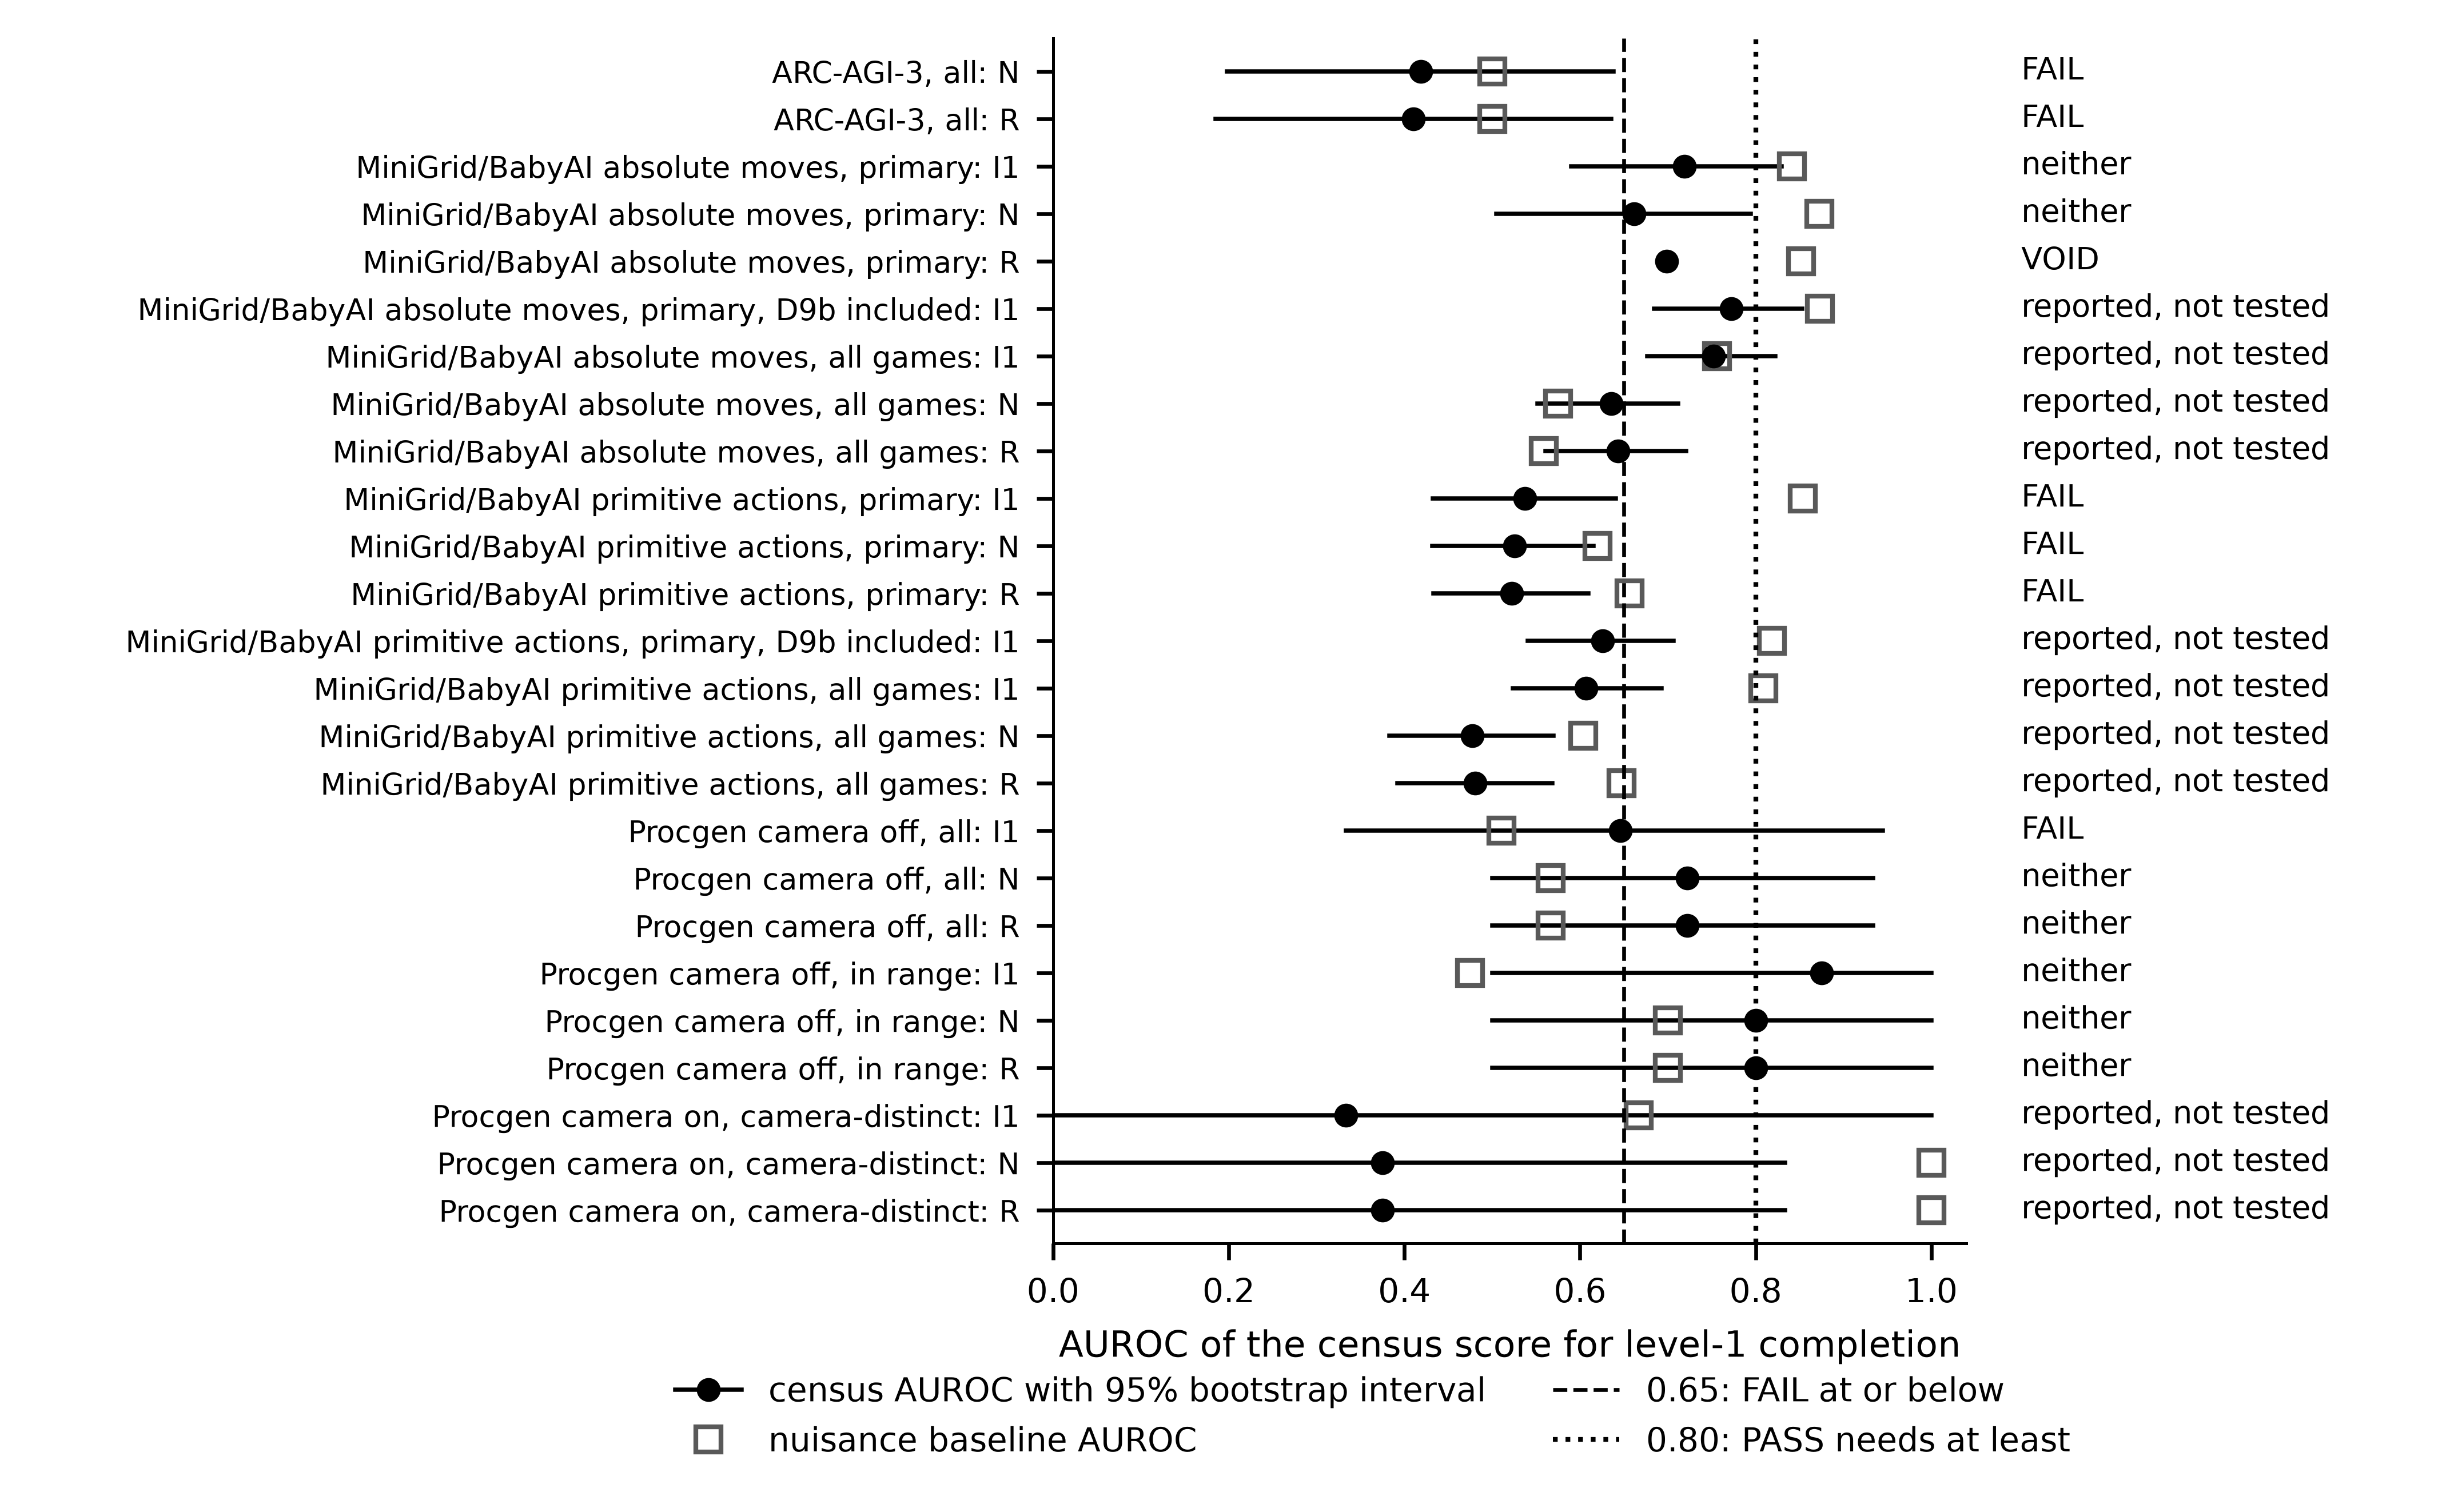
\includegraphics[width=\textwidth]{fig2.png}
\caption{Test V2: AUROC of the census score for first-level completion (filled
circle) with its 95\% bootstrap interval, and the AUROC of the nuisance
baseline (open square), per agent and line. Dashed line: 0.65, at or
below which V2 fails. Dotted line: 0.80, which V2 needs to pass, among
three further conditions. The word at the right is the verdict printed
by the frozen analysis code; the void line has no interval. The two
ARC-AGI-3 lines are reported and not tested, and the ``FAIL'' printed on
them has no registered meaning (Section III-J). The primitive-action
lines are reported by the registered text, so the ``FAIL'' printed on
their primary lines enters no outcome clause. ``Camera off'' is the
whole-level view and ``camera on'' the view centered on the agent;
``level-1 completion'' is first-level completion. Registered test; the
values are those of Supplement, Section S.2.}
\end{figure*}

\begin{table*}[!t]
\caption{Test V2, the verdict of each agent and the benchmark line, as printed by
the frozen analysis code at prereg-v1.1, for the tested lines, the
reported primitive-action line and the reported ARC-AGI-3 line. The
lines with excluded environments put back, the camera-on lines and every
statistic are in Supplement, Section S.2.}
\centering
\footnotesize
\renewcommand{\arraystretch}{1.15}
\setlength{\tabcolsep}{4pt}
\begin{tabular}{>{\raggedright\arraybackslash}p{0.322\linewidth}>{\raggedright\arraybackslash}p{0.082\linewidth}>{\raggedright\arraybackslash}p{0.082\linewidth}>{\raggedright\arraybackslash}p{0.124\linewidth}>{\raggedright\arraybackslash}p{0.301\linewidth}}
\hline
\textbf{line} & \textbf{R} & \textbf{I1} & \textbf{N (instrument check)} & \textbf{benchmark line} \\ \hline
MiniGrid/BabyAI, absolute moves, primary & VOID & neither & neither & not failed (decided by I1 alone) \\
MiniGrid/BabyAI, primitive actions, primary (reported) & FAIL & FAIL & FAIL & suite FAIL (decided by R and I1) \\
Procgen, whole-level view, all games & neither & FAIL & neither & not failed (decided by R and I1) \\
Procgen, whole-level view, in-range games & neither & neither & neither & not failed (decided by R and I1) \\
ARC-AGI-3, 25 public games (reported) & FAIL & not run & FAIL & reported, not tested \\
\hline
\end{tabular}
\end{table*}

Under absolute moves the MiniGrid/BabyAI benchmark line is ``not
failed'', decided by I1 alone because R is void, and Procgen with the
whole-level view is ``not failed'' over all games and over the in-range
games. The primitive-action line reads ``suite FAIL'', but the
registered text only reports that condition, so it enters no outcome
clause (Section III-J).

The nuisance baseline ranked the games better than the census on all six
primary MiniGrid/BabyAI lines: the three under absolute moves, which the
registered text tests, and the three under primitive actions, which it
reports (Fig. 2). Over all 14 MiniGrid/BabyAI lines, primary or not, the
baseline is higher on 12. The two exceptions are reported lines under
absolute moves with all games included, for N (census 0.6352, baseline
0.5752) and for R (census 0.6434, baseline 0.5589). On Procgen the
baseline is below the census on every line of the whole-level view.

The two ARC-AGI-3 lines are reported and not tested, as registered;
because of the defect recorded among the deviations, they are computed
over all 25 public games, and the ``FAIL'' printed on them has no
registered meaning and enters no gate.

Gate G3 applies the registered outcome table (Table III). The outcome is
a refutation, by the clause ``V1 fails on any suite'': V1 fails on
MiniGrid/BabyAI in both conditions and on Procgen. The other two clauses
of the refutation do not apply, since the V2 benchmark line under
absolute moves is ``not failed'' and V2 is not void on every benchmark.
One clause is enough. This classification was recorded on 13 October
2026, before any text about the results was written.

\begin{table*}[!t]
\caption{The registered outcome table, as fixed in the protocol before any
confirmatory run (B: MiniGrid/BabyAI; C: Procgen; B-macro:
MiniGrid/BabyAI under absolute moves).}
\centering
\footnotesize
\renewcommand{\arraystretch}{1.15}
\setlength{\tabcolsep}{4pt}
\begin{tabular}{>{\raggedright\arraybackslash}p{0.087\linewidth}>{\raggedright\arraybackslash}p{0.562\linewidth}>{\raggedright\arraybackslash}p{0.285\linewidth}}
\hline
\textbf{outcome} & \textbf{definition (registered)} & \textbf{venue (registered)} \\ \hline
Support & V1 passes on B (both conditions) and C, V2 passes for R and I1 on
B-macro and C (not void), and V3 holds & JAIR full article \\
Partial & V1 passes everywhere, but V2 passes on B-macro only or is void on C, or
passes on C for R only & IEEE Transactions on Games full paper \\
Refute & V1 fails on any suite, or V2 fails on B-macro, or V2 is void on every
suite & repository record only, at most an arXiv note \\
\hline
\end{tabular}
\end{table*}

\section{Exploratory Diagnosis}\label{exploratory-diagnosis}

This section is exploratory. It asks why an instrument with fixed
parameters did not keep its meaning across benchmarks; it was written
after the outcome was known, tests nothing, and changes nothing above.
Its numbers come from an exploratory script that calls the frozen
analysis functions unchanged (Supplement, Section S.5); the census
verdict stored in each of the 3,500 planner rows equals the verdict
recomputed from that row's report, with 0 mismatches. Fig. 3 shows, for
every V1 line, how the games split between truth and census, and Fig. 4
how often single seeds disagree with their game's majority. Both are
exploratory.

\begin{figure*}[!t]
\centering
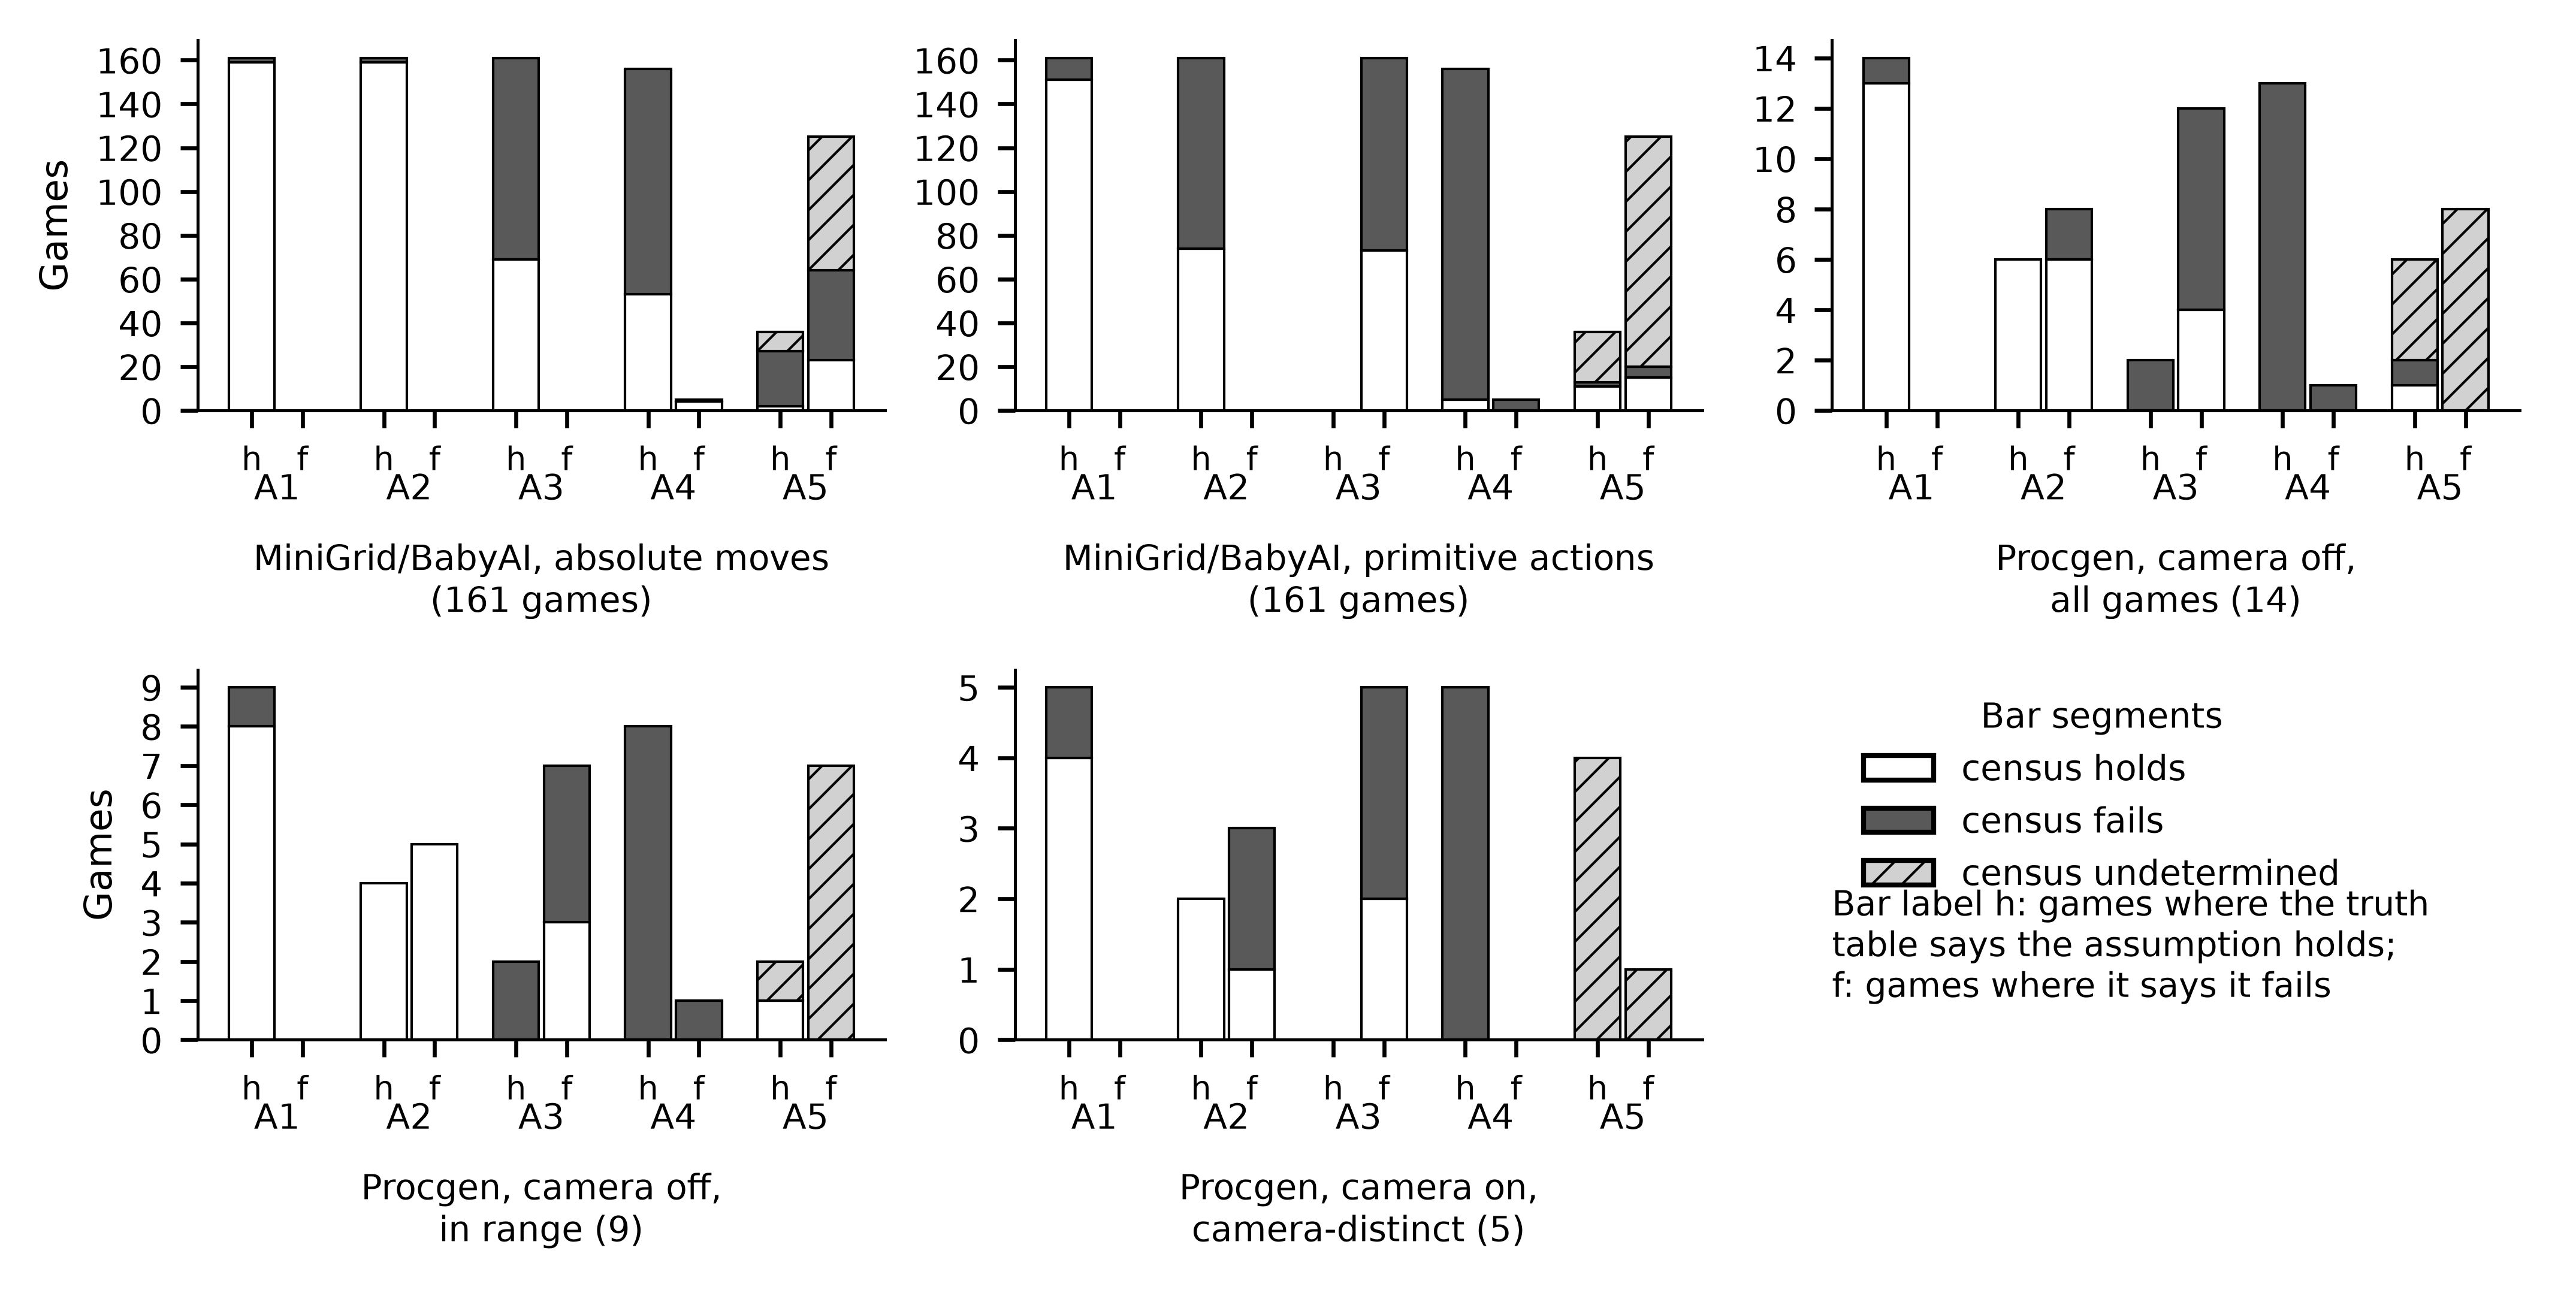
\includegraphics[width=\textwidth]{fig3.png}
\caption{An exploratory view of V1: for each benchmark and condition and each
assumption, the games where the truth table says the assumption holds
(bar h) or fails (bar f), split by the census verdict (holds, fails,
undetermined). A missing bar is a truth class with zero games. ``Camera
off'' is the whole-level view and ``camera on'' the view centered on the
agent. Exploratory, read after the outcome was known; source in
Supplement, Section S.5.}
\end{figure*}

In this exploratory reading, for A1 the census agrees with the truth on
151 of 161 games under primitive actions, 159 of 161 under absolute
moves and 13 of 14 on Procgen; every disagreement is a game where the
truth holds and the census fails. For A2 under primitive actions, 87
games have the truth holding and the census failing. On their 870 seeds
the two turn keys were recorded as producing no movement on all 870: a
turn changes the agent's facing but not its cell, and the adapter merges
the four facings into one tile index, so a turn changes nothing the
census can see. Under absolute moves A2 agrees on 159 of 161 games. On 6
Procgen games the truth fails A2, because other entities also respond to
the action, and the census says it holds; the census rule has no clause
for that.

For A3 under absolute moves, 92 games have the truth holding and the
census failing. Four step vectors were accepted on 850 of their 920
seeds, so the learned motion was mostly right; of the 775 seeds whose
verdict is ``fails'', 755 carry the planner's first-level outcome
``mispredicted''. The census's A3 failure therefore comes from the
planner's prediction during play, not from the learned step vectors.
Under primitive actions the truth fails everywhere, and the census says
``holds'' on 73 games. The census rule for A4 is conditional on A3, so
most A4 failures on MiniGrid/BabyAI follow from those of A3; on Procgen
the counter of walked-through ``walls'' is above zero on some seeds of
all 13 games where the truth holds A4.

For A5, the exploratory counts show that most seeds with an undetermined
verdict never recorded a goal place at all: 620 of 663 under absolute
moves, 986 of 1,074 under primitive actions and 70 of 110 on Procgen. A
place is recorded only at a level end, so on these seeds the census had
nothing to test. The census said ``holds'' where the truth fails on 23
games under absolute moves and 15 under primitive actions; success there
needs facing the target, a toggle or a pickup, the level ends on a cell
beside or in front of the target, and the census, reading places only,
recorded that cell as a goal. The negative kappa values for A5 come
mostly from ``undetermined'', which the registered kappa maps to the
value opposite the truth. The cell ``truth fails, census holds'' used by
kappa therefore contains 23 census ``holds'' and 61 undetermined games
under absolute moves (84 in all), 15 and 105 under primitive actions
(120 in all), and 0 and 8 on Procgen (8 in all).

\begin{figure*}[!t]
\centering
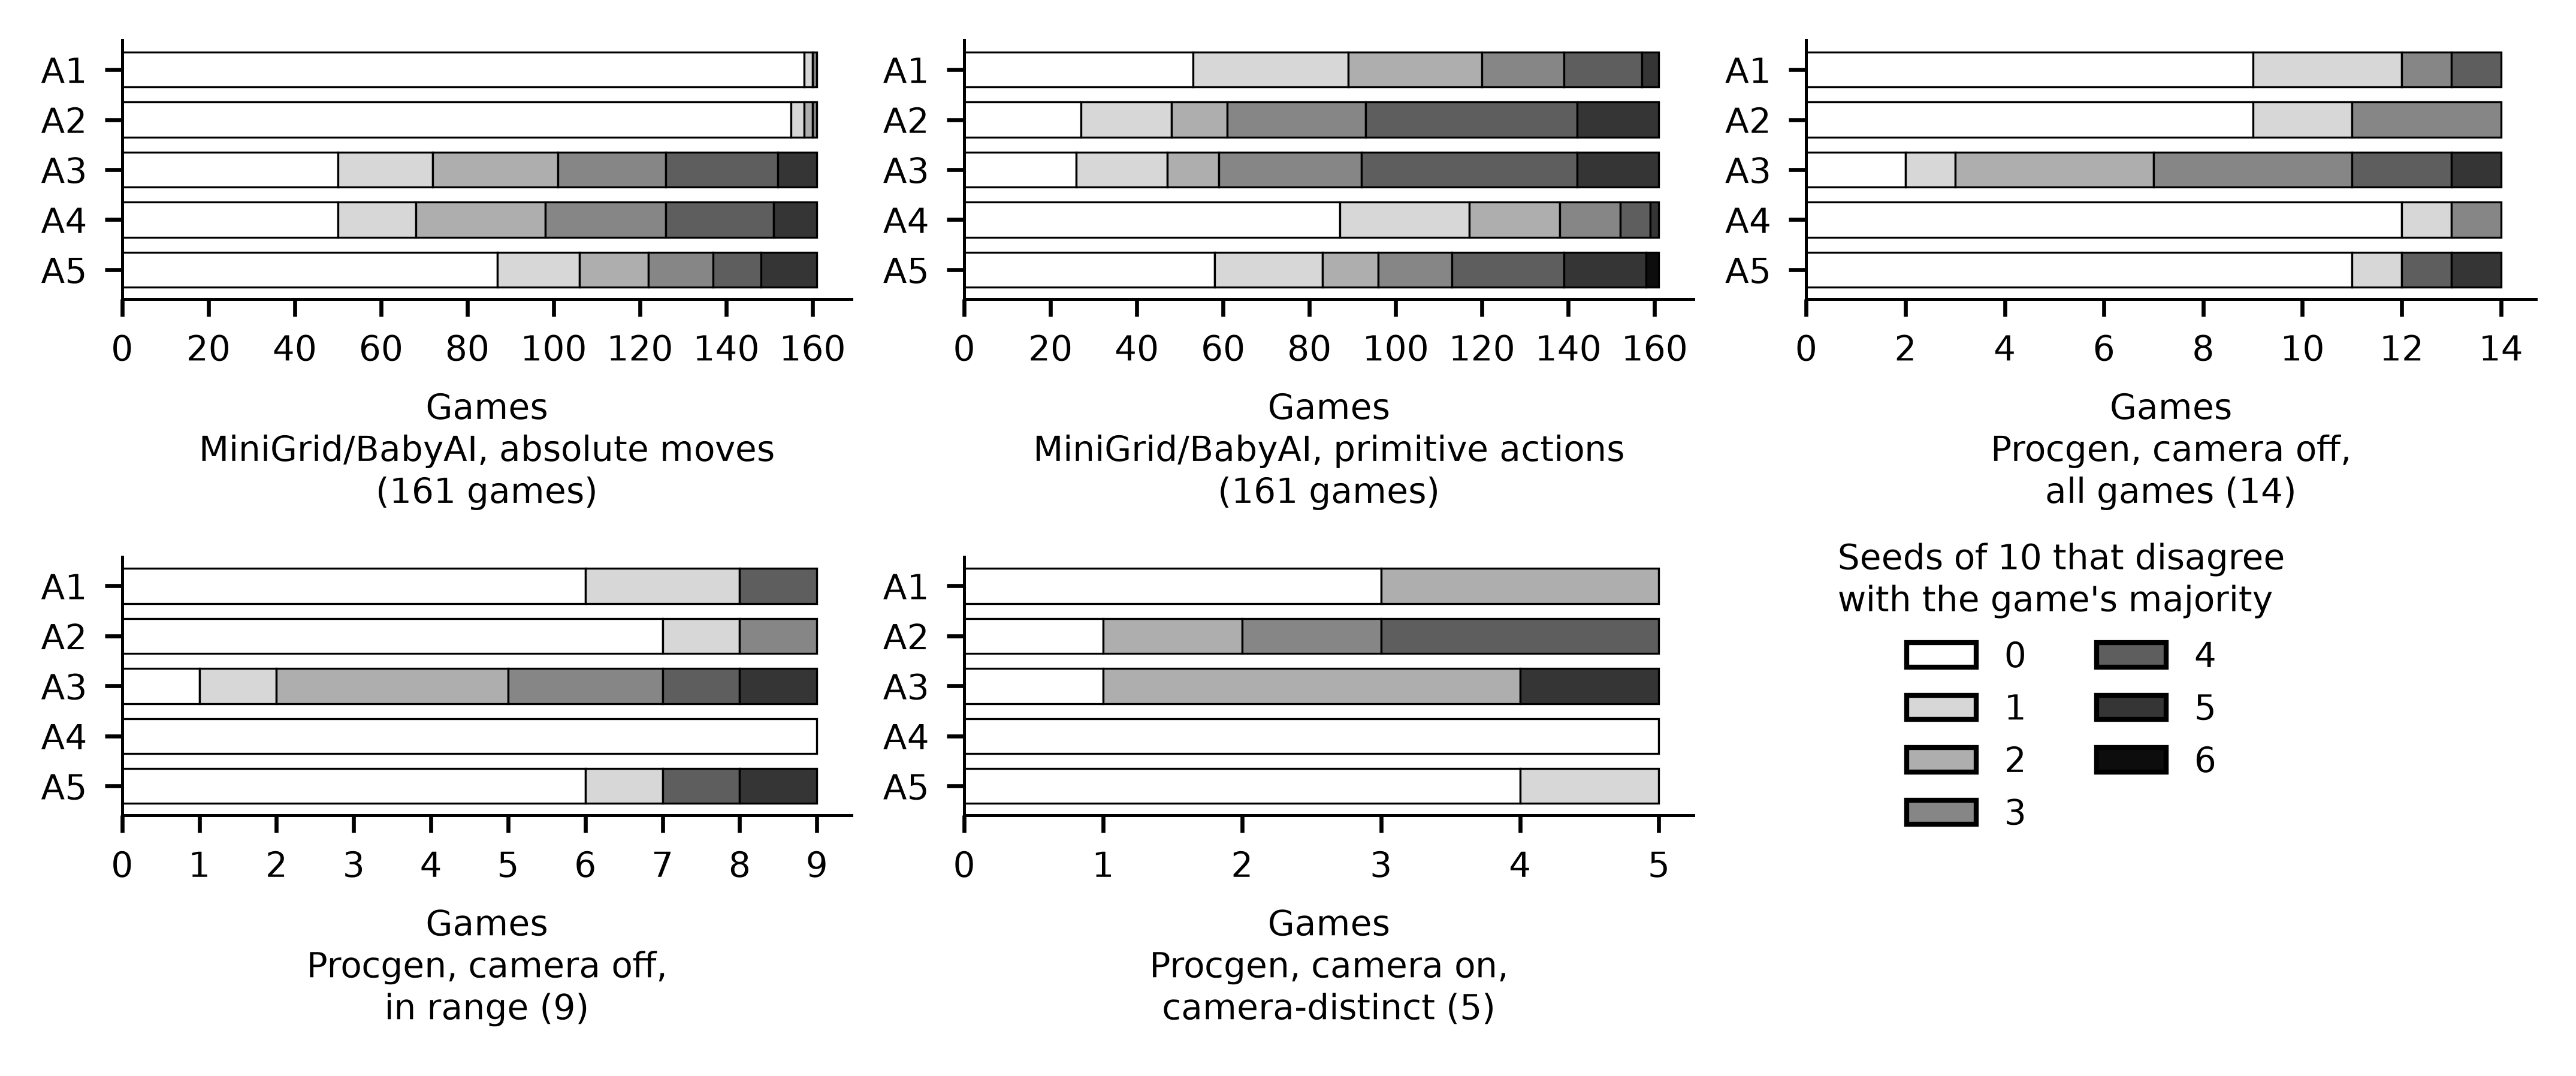
\includegraphics[width=\textwidth]{fig4.png}
\caption{An exploratory view of seed dissent: for each benchmark and condition
and each assumption, the games split by how many of their 10 seeds give
a census verdict different from the game's majority verdict. ``Camera
off'' is the whole-level view and ``camera on'' the view centered on the
agent. Exploratory, read after the outcome was known; source in
Supplement, Section S.5.}
\end{figure*}

Seeds often disagree with their game's majority where the verdict
depends on the course of the planner's run (Fig. 4): at least one seed
dissents on 134 of 161 games for A2 under primitive actions, 135 for A3
under primitive actions, and 111 each for A3 and A4 under absolute
moves, but only on 3 and 6 games for A1 and A2 under absolute moves.

The exploratory reading that ties these counts together concerns
constructs. For A2 under primitive actions, and for A3, A4 and A5, the
census probe and the truth definition are not the same construct. The
census A2 asks whether some key moves one located object; the truth asks
whether exactly one object's displacement is a fixed function of the
action, turns included. The census A3 asks whether the planner's
first-level model mispredicted; the truth asks whether each action's
unblocked displacement is constant. The census A4 counts walked-through
``wall'' colors; the truth asks whether every blocked move is explained
by a fixed obstacle set. The census A5 is silent when no level ends; the
truth asks whether success is triggered by entering a place. In each
case the census reads a by-product of one planner's run, while the truth
reads the environment's step function. This is a description of the
mismatch, made after the outcome, not a fix and not a result. On the 17
held-out ARC-AGI-3 games, the exploratory V2 line computed by the same
frozen functions gives AUROC 0.3542 for N and 0.3403 for R (Supplement,
Section S.7); it is reported and never tested. None of this exploratory
material supports a causal claim; these are counts of counters, read
after the outcome was known.

\section{Discussion}\label{discussion}

The registered answer is no on both counts: the census failed the
registered validity test on games from the two other benchmarks, and its
score passed the registered prediction test for no agent there.

\subsection{What the Failure Means}\label{what-the-failure-means}

The truth table is the registered answer key, committed before
registration with the source line behind each entry; the census verdict
is the instrument under test. A failing V1 line therefore says that the
census as registered does not measure that assumption on that benchmark.
A V1 failure on any benchmark decides the outcome by itself, and a
prediction built on a score that does not measure what it names would be
hard to interpret even if it had passed.

The census kept every parameter fixed across benchmarks, which was the
registered meaning of transfer, and it still failed. Holding parameters
fixed is a statement about the procedure, not about whether it measures
the same property on new games. If intelligence is defined over a range
of environments {[}8{]}, a claim that an instrument describes games in
general is a claim about a range too, to be tested on each part of the
range it names; and an instrument that characterizes games carries
priors of its own {[}9{]}, here the planner whose by-products the census
read. The registered decision rule worked as designed, and no reading of
the results after the fact could turn the refutation into support.

\subsection{Why the Failure Could Not Show on the Development
Benchmark}\label{why-the-failure-could-not-show-on-the-development-benchmark}

I set the census constants while developing the planner on eight
ARC-AGI-3 games, and I wrote the per-seed rules on top of the planner's
report. I never wrote the registered development truth table for those
games, so V1 was never computed there. The census was tuned to make the
planner work, and nothing on ARC-AGI-3 measured whether its verdicts
matched the games' mechanics, so a disagreement could not show there.
The registered phrase that ARC-AGI-3 ``does not count toward
generality'' kept the development games out of the evidence for the
claim, not out of that check.

\subsection{The Pilot Check That Was Not
Done}\label{the-pilot-check-that-was-not-done}

The pilot runs contained census verdicts for eight games with
truth-table entries, six MiniGrid/BabyAI environments and two Procgen
games. Comparing them with the truth before the v1.1 tag could have
shown the disagreement before the 10,500 confirmatory runs were made;
the protocol did not register such a check, and I did not make one.
Since the pilot could change adapter code but no census constant,
threshold or truth entry, an early warning could not have rescued the
claim, but it would have changed what was run next.

\subsection{The Nuisance Baseline}\label{the-nuisance-baseline}

The baseline is fitted in-sample and the census score is not fitted to
the outcome at all, so the comparison favors the baseline; it is the
comparison the protocol registered. For the agents and conditions
examined, how large and how varied a MiniGrid/BabyAI environment is
predicted first-level completion better than the five assumptions as
measured. That is a statement about the measured census, not about the
assumptions as properties of the games.

\subsection{The Methodological
Mistake}\label{the-methodological-mistake}

The reason the census did not carry over is a mistake of method, read
from the exploratory diagnosis: the probes and the truth predicates were
not the same constructs, and no test existed where the parameters were
set. The census decisions were by-products of one planner's run; the
truth entries are properties of the environment's step function. Only A1
is measured in nearly the same terms on both sides, and only A1 had no
failing V1 line. I wrote the truth definitions and the census rules
separately and never checked on any game, before registration, that one
estimated the other.

\subsection{What a Second Registered Study Would Have to
Change}\label{what-a-second-registered-study-would-have-to-change}

These are requirements for a different study, not a result and not an
existing instrument. It would have to define each probe and its truth
predicate as the same construct, write a truth table for the development
instance and compute V1 there, all before registration; register a V1
gate with a stop rule on the pilot games of every benchmark; register
how ``undetermined'' enters each test, so that a silent instrument and a
wrong one are told apart; and name in advance a nuisance baseline that
the census must beat on the development instance.

\subsection{What This Study Does Not
Show}\label{what-this-study-does-not-show}

This study says nothing about the ability of frame-only agents on these
games, and it does not show that A1 to A5 are poor descriptions of the
games; the truth tables say how often each holds. It says nothing about
the hidden ARC-AGI-3 games or about agents that bring priors to the
games. It does not show that a differently built census would fail, or
that instruments built on one benchmark cannot transfer to others. It
shows that this instrument, registered with these thresholds, did not.

\section{Conclusion}\label{conclusion}

The registered objective was a frame-only census, built and frozen on
ARC-AGI-3, that would report the mechanics of games from other
benchmarks at a registered accuracy and predict where assumption-driven
agents complete the first level. It failed in each registered respect:
V1 failed on both confirmatory benchmarks, for three or four of the five
assumptions depending on the benchmark and condition; V2 passed for no
agent on any benchmark; and on MiniGrid/BabyAI a baseline built from the
size and variety of the environments ranked them better than the census
did. The registered consequence followed: a refutation. For anyone who
builds an instrument on one benchmark to describe the games of another,
the record here is that freezing the parameters secured nothing about
validity, and that the check that could have shown the failure, a
comparison with known truth on the development and pilot games, was
never run.

\section*{Data and Code Availability}\label{data-and-code-availability}
\addcontentsline{toc}{section}{Data and Code Availability}

All data and code are public under the MIT license in a repository whose
address is withheld for double-anonymous review; an anonymized copy for
reviewers is at {[}ANONYMIZED REPOSITORY URL{]}. The data are the 10,500
confirmatory rows, one JSON file per benchmark, condition, agent, game
and seed, the 500-row ARC-AGI-3 baseline, the pilot rows, the outputs of
the four checks, the analysis logs and the V1 and V2 tables. The code is
every script that produced them and the scripts that build and check
this article's numbers and figures; the agent I1 keeps the upstream MIT
notice of its authors. The registered protocol is at the tags prereg-v1,
prereg-v1.1 and prereg-v1.2, and the two OSF registrations are public.
An earlier version of this article and the supplement are on Zenodo
under CC-BY 4.0. Commit hashes, registration addresses and the two
Zenodo identifiers are withheld for review and given to the
Editor-in-Chief.

\section*{Funding and Conflicts of
Interest}\label{funding-and-conflicts-of-interest}
\addcontentsline{toc}{section}{Funding and Conflicts of Interest}

This research received no funding. The author declares no conflicts of
interest.

\begin{thebibliography}{99}
\bibitem{b1}
D. Perez-Liebana \emph{et al.}, ``The 2014 General Video Game Playing
Competition,'' \emph{IEEE Trans. Comput. Intell. AI Games}, vol.~8, no.
3, pp.~229--243, Sep.~2016, doi: 10.1109/TCIAIG.2015.2402393.

\bibitem{b2}
ARC Prize Foundation, ``ARC-AGI-3: A new challenge for frontier agentic
intelligence,'' Tech. Rep., Apr.~22, 2026. Accessed: Oct.~24, 2026.
{[}Online{]}. Available:
\url{https://arcprize.org/media/ARC_AGI_3_Technical_Report.pdf}

\bibitem{b3}
M. Chevalier-Boisvert \emph{et al.}, ``Minigrid \& Miniworld: Modular \&
customizable reinforcement learning environments for goal-oriented
tasks,'' in \emph{Advances in Neural Inf. Process. Syst.}, vol.~36,
2023, pp.~73383--73394, doi: 10.52202/075280-3209.

\bibitem{b4}
M. Chevalier-Boisvert \emph{et al.}, ``BabyAI: A platform to study the
sample efficiency of grounded language learning,'' in \emph{Proc. Int.
Conf. Learn. Representations}, 2019. {[}Online{]}. Available:
\url{https://openreview.net/forum?id=rJeXCo0cYX}

\bibitem{b5}
K. Cobbe, C. Hesse, J. Hilton, and J. Schulman, ``Leveraging procedural
generation to benchmark reinforcement learning,'' in \emph{Proc. 37th
Int. Conf. Mach. Learn.}, H. Daumé III and A. Singh, Eds., Proc. Mach.
Learn. Res., vol.~119, 2020, pp.~2048--2056. {[}Online{]}. Available:
\url{https://proceedings.mlr.press/v119/cobbe20a.html}

\bibitem{b6}
M. Genesereth, N. Love, and B. Pell, ``General game playing: Overview of
the AAAI competition,'' \emph{AI Mag.}, vol.~26, no. 2, pp.~62--72,
2005, doi: 10.1609/aimag.v26i2.1813.

\bibitem{b7}
D. Perez-Liebana, J. Liu, A. Khalifa, R. D. Gaina, J. Togelius, and S.
M. Lucas, ``General Video Game AI: A multitrack framework for evaluating
agents, games, and content generation algorithms,'' \emph{IEEE Trans.
Games}, vol.~11, no. 3, pp.~195--214, Sep.~2019, doi:
10.1109/TG.2019.2901021.

\bibitem{b8}
S. Legg and M. Hutter, ``Universal intelligence: A definition of machine
intelligence,'' \emph{Minds and Machines}, vol.~17, no. 4, pp.~391--444,
2007, doi: 10.1007/s11023-007-9079-x.

\bibitem{b9}
F. Chollet, ``On the measure of intelligence,'' 2019, arXiv:1911.01547.

\bibitem{b10}
P. Bontrager, A. Khalifa, A. Mendes, and J. Togelius, ``Matching games
and algorithms for general video game playing,'' in \emph{Proc. AAAI
Conf. Artif. Intell. Interactive Digit. Entertainment}, vol.~12, no. 1,
2016, pp.~122--128, doi: 10.1609/aiide.v12i1.12884.

\bibitem{b11}
R. D. Gaina, S. M. Lucas, and D. Perez-Liebana, ``General win prediction
from agent experience,'' in \emph{Proc. 2018 IEEE Conf. Comput. Intell.
Games (CIG)}, 2018, pp.~1--8, doi: 10.1109/CIG.2018.8490439.

\bibitem{b12}
C. Laidlaw, S. J. Russell, and A. Dragan, ``Bridging RL theory and
practice with the effective horizon,'' in \emph{Advances in Neural Inf.
Process. Syst.}, vol.~36, 2023, pp.~58953--59007, doi:
10.52202/075280-2573.

\bibitem{b13}
E. Rudakov, J. Shock, and B. U. Cowley, ``Graph-based exploration for
ARC-AGI-3 interactive reasoning tasks,'' 2025, arXiv:2512.24156.

\bibitem{b14}
K. H. Liew, ``Explore before you solve: The speed--depth trade-off in
epistemic agents for ARC-AGI-3,'' 2026, arXiv:2605.25931.

\bibitem{b15}
A. Skoutnev, K. Acharya, G. Longhitano, M. Udell, K. Ellis, and I.
Drori, ``Twin: Playing an unknown game with a test-time digital twin,''
2026, arXiv:2608.14490.

\bibitem{b16}
M. G. Bellemare, J. Veness, and M. Bowling, ``Investigating contingency
awareness using Atari 2600 games,'' in \emph{Proc. AAAI Conf. Artif.
Intell.}, vol.~26, no. 1, 2012, pp.~864--871, doi:
10.1609/aaai.v26i1.8321.

\bibitem{b17}
J. Choi \emph{et al.}, ``Contingency-aware exploration in reinforcement
learning,'' in \emph{Proc. Int. Conf. Learn. Representations}, 2019.
{[}Online{]}. Available:
\url{https://openreview.net/forum?id=HyxGB2AcY7}

\bibitem{b18}
A. Blum and M. Hardt, ``The Ladder: A reliable leaderboard for machine
learning competitions,'' in \emph{Proc. 32nd Int. Conf. Mach. Learn.},
F. Bach and D. Blei, Eds., Proc. Mach. Learn. Res., vol.~37, 2015,
pp.~1006--1014. {[}Online{]}. Available:
\url{https://proceedings.mlr.press/v37/blum15.html}

\bibitem{b19}
R. Roelofs \emph{et al.}, ``A meta-analysis of overfitting in machine
learning,'' in \emph{Advances in Neural Inf. Process. Syst.}, vol.~32,
2019. {[}Online{]}. Available:
\url{https://papers.nips.cc/paper_files/paper/2019/hash/ee39e503b6bedf0c98c388b7e8589aca-Abstract.html}

\bibitem{b20}
L. Bertinetto, J. F. Henriques, S. Albanie, M. Paganini, and G. Varol,
``Preface,'' in \emph{NeurIPS 2020 Workshop on Pre-registration in
Machine Learning}, L. Bertinetto, J. F. Henriques, S. Albanie, M.
Paganini, and G. Varol, Eds., Proc. Mach. Learn. Res., vol.~148, 2021,
p.~i. {[}Online{]}. Available:
\url{https://proceedings.mlr.press/v148/bertinetto21a.html}

\bibitem{b21}
S. A. Goldman and M. J. Kearns, ``On the complexity of teaching,''
\emph{J. Comput. Syst. Sci.}, vol.~50, no. 1, pp.~20--31, 1995, doi:
10.1006/jcss.1995.1003.

\bibitem{b22}
T. M. Mitchell, ``Generalization as search,'' \emph{Artif. Intell.},
vol.~18, no. 2, pp.~203--226, 1982, doi: 10.1016/0004-3702(82)90040-6.

\bibitem{b23}
S. Keren, A. Gal, and E. Karpas, ``Goal recognition design,'' in
\emph{Proc. Int. Conf. Automated Planning and Scheduling}, vol.~24, no.
1, 2014, pp.~154--162, doi: 10.1609/icaps.v24i1.13617.

\bibitem{b24}
C. Wayllace, P. Hou, W. Yeoh, and T. C. Son, ``Goal recognition design
with stochastic agent action outcomes,'' in \emph{Proc. 25th Int. Joint
Conf. Artif. Intell. (IJCAI-16)}, 2016, pp.~3279--3285. {[}Online{]}.
Available: \url{https://www.ijcai.org/Proceedings/16/Papers/464.pdf}
\end{thebibliography}
\end{document}
